\documentclass{beamer}
\begin{document}
\title{KiCAD\\Creating a component footprint}
\author{Katharina Fey}
\date{17. March 2018}

\frame{\titlepage}

%%%%%%%%%%%%%%%%%%%%%%%%%%%%%%%%%%%%%%%%%%%%%%%%%%%%%%%%%
\begin{frame}
  \frametitle{Create new footprint}
  \begin{itemize}
    \item Open the footprint editor and create a new footprint
    \item Alternatively: load an existing library and add/ clone a footprint there
  \end{itemize}
  \begin{figure}[H]
    \centering
    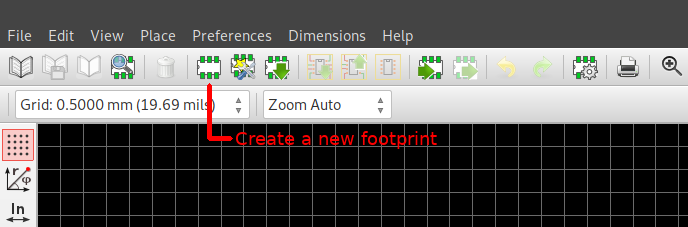
\includegraphics[width=0.85\textwidth]{images/step_01.png}
  \end{figure}
\end{frame}


%%%%%%%%%%%%%%%%%%%%%%%%%%%%%%%%%%%%%%%%%%%%%%%%%%%%%%%%%
\begin{frame}
  \frametitle{Create new footprint}
  \begin{figure}[H]
    \centering
    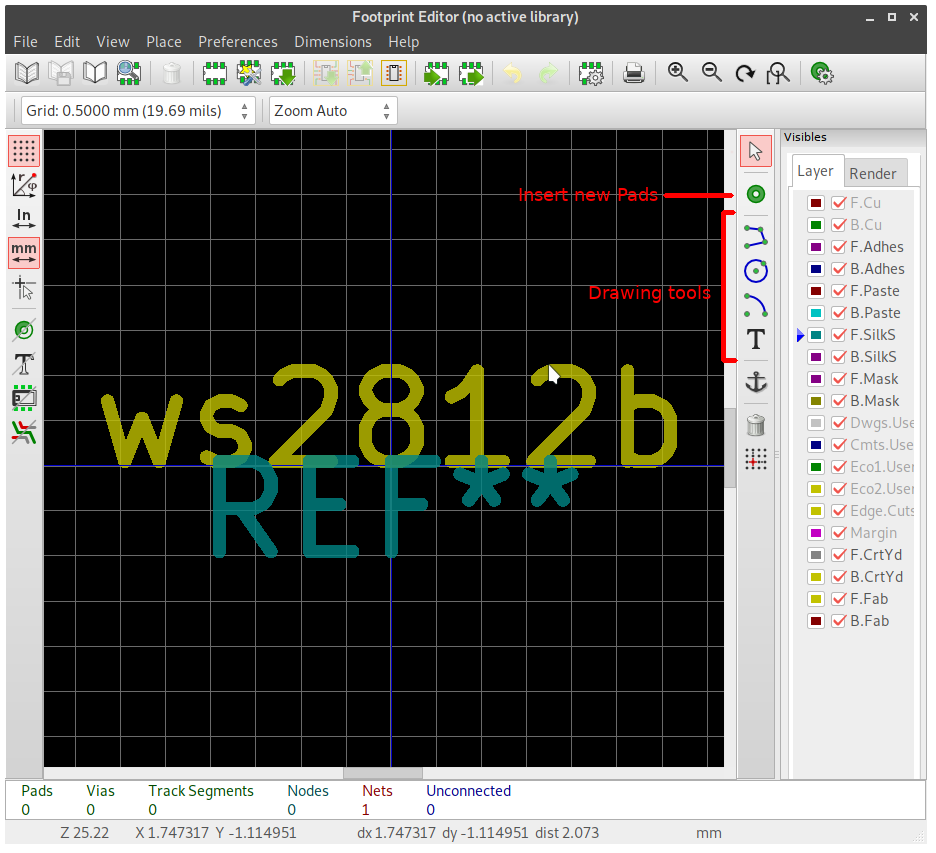
\includegraphics[width=0.55\textwidth]{images/step_02.png}
  \end{figure}
\end{frame}


%%%%%%%%%%%%%%%%%%%%%%%%%%%%%%%%%%%%%%%%%%%%%%%%%%%%%%%%%
\begin{frame}
  \frametitle{Set custom grid}
  \begin{itemize}
    \item It's easier to align pads \& marks on a custom grid size
  \end{itemize}
  \begin{figure}[H]
    \centering
    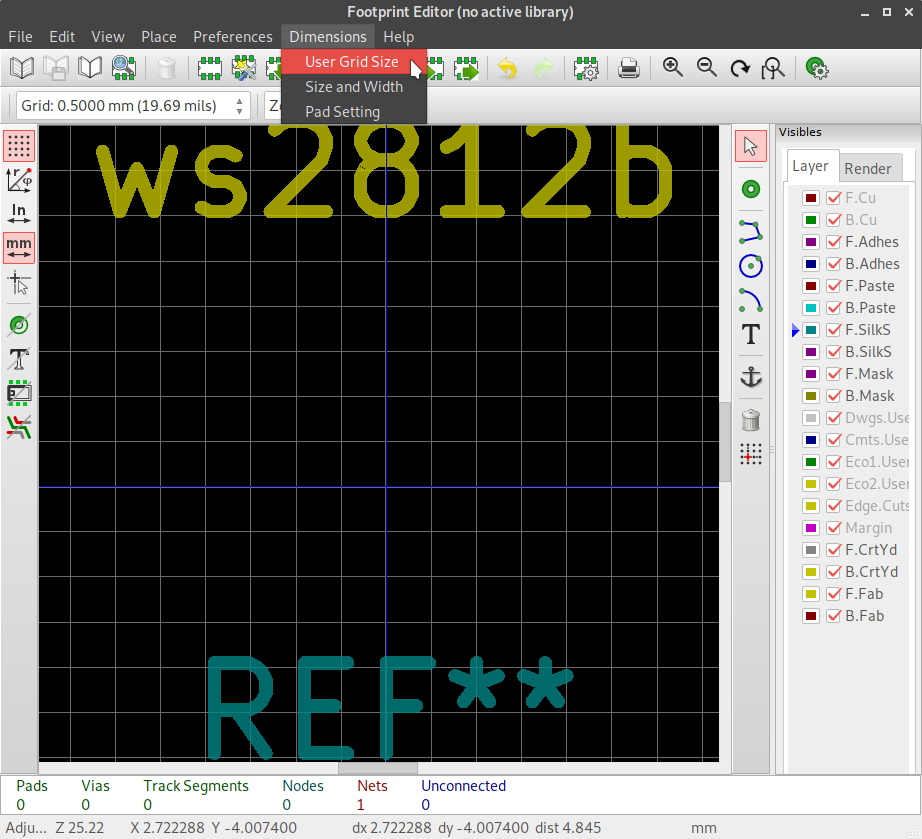
\includegraphics[width=0.65\textwidth]{images/step_03.png}
  \end{figure}
\end{frame}


%%%%%%%%%%%%%%%%%%%%%%%%%%%%%%%%%%%%%%%%%%%%%%%%%%%%%%%%%
\begin{frame}
  \frametitle{Set custom grid}
  \begin{itemize}
    \item Look at useful dimensions from the datasheet
    \item Half those dimensions and set them as the grid-sizes
  \end{itemize}
  \begin{figure}[H]
    \centering
    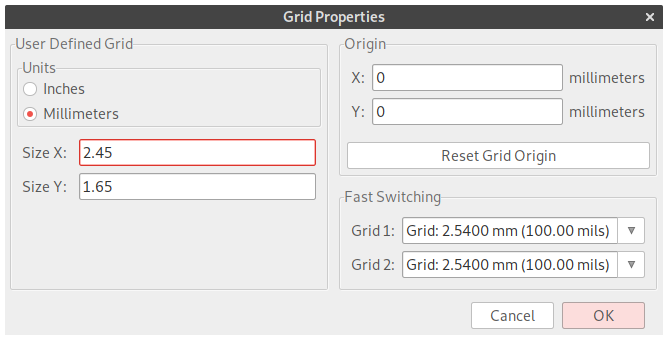
\includegraphics[width=0.85\textwidth]{images/step_04.png}
  \end{figure}
\end{frame}


%%%%%%%%%%%%%%%%%%%%%%%%%%%%%%%%%%%%%%%%%%%%%%%%%%%%%%%%%
\begin{frame}
  \frametitle{Create \& customise Pads}
  \begin{itemize}
    \item Select the custom grid
    \item Then select the pad-tool and place a pad
    \item Hover over the pad and press `e' to edit it's dimensions
  \end{itemize}
\end{frame}


%%%%%%%%%%%%%%%%%%%%%%%%%%%%%%%%%%%%%%%%%%%%%%%%%%%%%%%%%
\begin{frame}
  \frametitle{Create \& customise Pads}
  \begin{itemize}
    \item Set the pad type (SMD \& Through-Hole most common)
    \item Define the pad size \& optionally drill sizes
  \end{itemize}
  \begin{figure}[H]
    \centering
    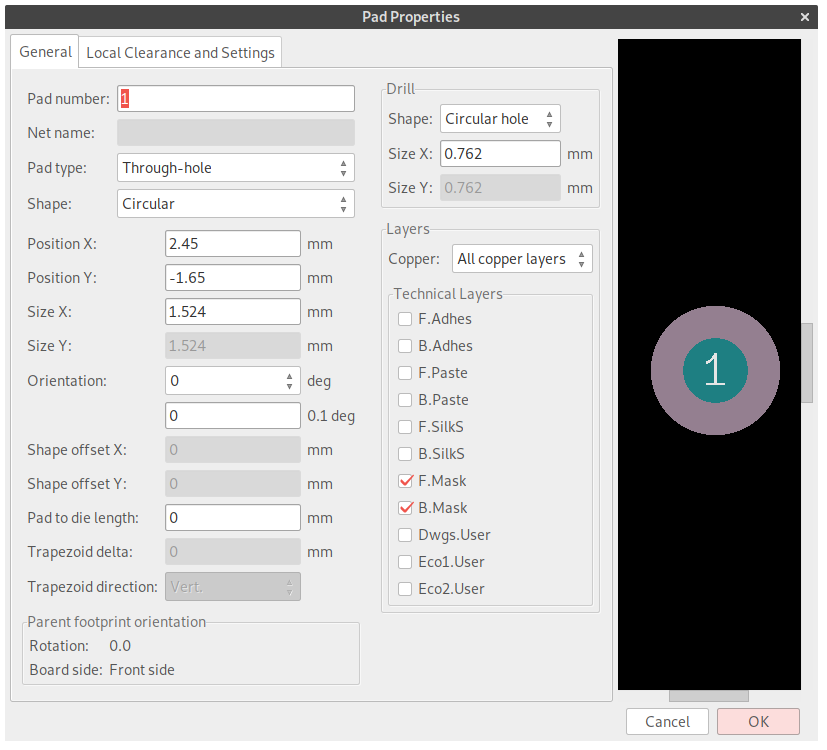
\includegraphics[width=0.55\textwidth]{images/step_05.png}
  \end{figure}
\end{frame}


%%%%%%%%%%%%%%%%%%%%%%%%%%%%%%%%%%%%%%%%%%%%%%%%%%%%%%%%%
\begin{frame}
  \frametitle{Design the footprint}
  \begin{itemize}
    \item Place the pads according to the footprint datasheet
    \item Use the `Fab' layers to draw part outlines – won't be included on the PCB
    \item Use the `SilkS' layers to add markings for the PCB
    \begin{itemize}
      \item Reference marker (included by default)
      \item Orientation markers
      \item Additional outline information
    \end{itemize}
  \end{itemize}
  \begin{figure}[H]
    \centering
    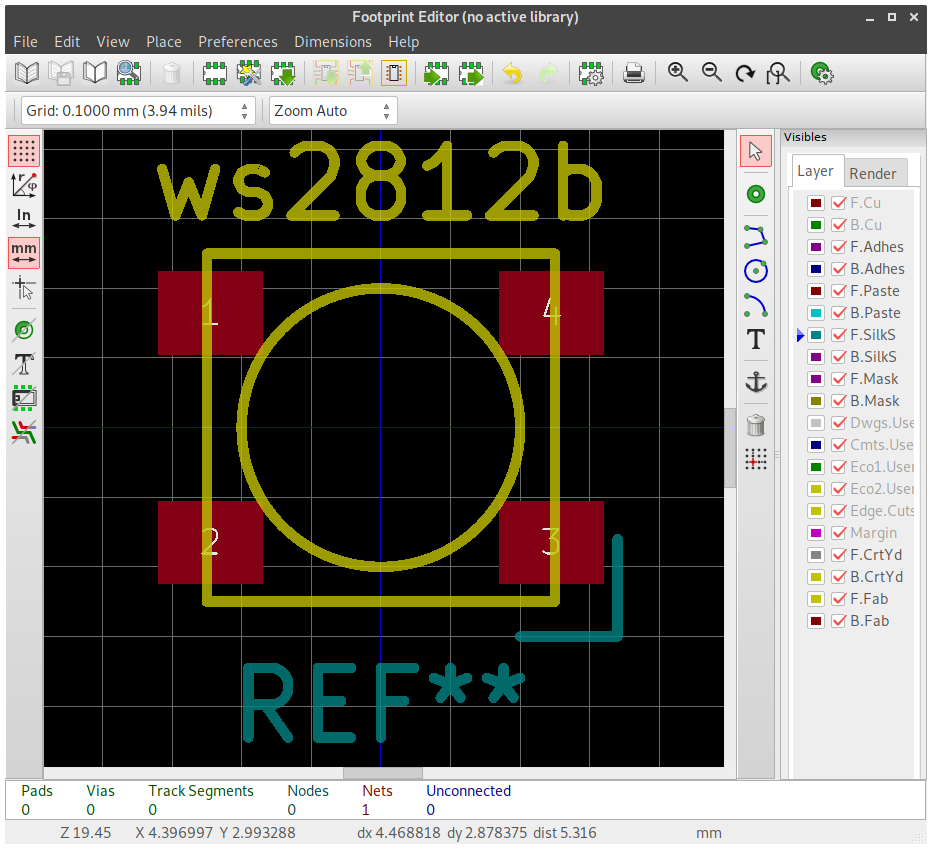
\includegraphics[width=0.45\textwidth]{images/step_06.png}
  \end{figure}
\end{frame}


%%%%%%%%%%%%%%%%%%%%%%%%%%%%%%%%%%%%%%%%%%%%%%%%%%%%%%%%%
\begin{frame}
  \frametitle{Save \& include new library}
  \begin{itemize}
    \item Save the footprint into a new library
    \item Then use the library wizard to include it
    \item Optionally: Tweak parameters in the Library Manager
  \end{itemize}
  \begin{figure}[H]
    \centering
    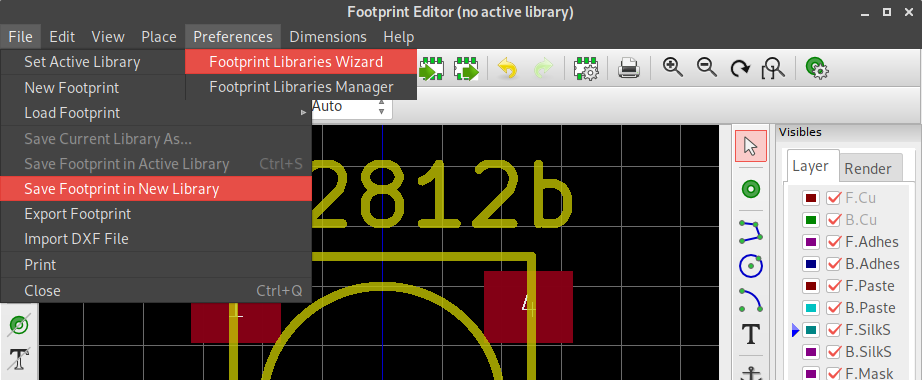
\includegraphics[width=0.85\textwidth]{images/step_07_08.png}
  \end{figure}
\end{frame}

\end{document}

